%%% Template originaly created by Karol Kozioł (mail@karol-koziol.net) and modified for ShareLaTeX use

\documentclass[a4paper,10pt]{article}

\usepackage[T1]{fontenc}
\usepackage[utf8]{inputenc}
\usepackage{graphicx}
\usepackage{xcolor}

%\renewcommand\familydefault{\sfdefault}
\usepackage{lmodern}
\usepackage{booktabs}
\usepackage{amsmath,amssymb,amsthm,textcomp}
\usepackage{enumerate}
\usepackage{multicol}
\usepackage{tikz}

\usepackage{geometry}
\geometry{left=20mm,right=20mm,%
bindingoffset=0mm, top=15mm,bottom=15mm}


\linespread{1}

\newcommand{\linia}{\rule{\linewidth}{0.5pt}}

% custom theorems if needed
\newtheoremstyle{mytheor}
    {1ex}{1ex}{\normalfont}{0pt}{\scshape}{.}{1ex}
    {{\thmname{#1 }}{\thmnumber{#2}}{\thmnote{ (#3)}}}

\theoremstyle{mytheor}
\newtheorem{defi}{Definition}

% my own titles
\makeatletter
\renewcommand{\maketitle}{
\begin{center}
\vspace{2ex}
{\huge \textsc{\@title}}
\vspace{1ex}
\\
\linia\\
\@author \hfill \@date
\vspace{1ex}
\end{center}
}
\makeatother
%%%

% custom footers and headers
\usepackage{fancyhdr}
\pagestyle{fancy}
\lhead{}
\chead{}
\rhead{}
\lfoot{CID: 01343907}
\cfoot{Time Series Analysis Coursework}
\rfoot{Page \thepage}
\renewcommand{\headrulewidth}{0pt}
\renewcommand{\footrulewidth}{0.5pt}
%

% code listing settings
\usepackage{listings}
\lstset{
    language=Python,
    basicstyle=\ttfamily\small,
    aboveskip={1.0\baselineskip},
    belowskip={1.0\baselineskip},
    columns=fixed,
    extendedchars=true,
    breaklines=true,
    tabsize=4,
    prebreak=\raisebox{0ex}[0ex][0ex]{\ensuremath{\hookleftarrow}},
    frame=lines,
    showtabs=false,
    showspaces=false,
    showstringspaces=false,
    keywordstyle=\color[rgb]{0.627,0.126,0.941},
    commentstyle=\color[rgb]{0.133,0.545,0.133},
    stringstyle=\color[rgb]{01,0,0},
    numbers=left,
    numberstyle=\small,
    stepnumber=1,
    numbersep=10pt,
    captionpos=t,
    escapeinside={\%*}{*)}
}

%%%----------%%%----------%%%----------%%%----------%%%

\begin{document}

\title{Time Series Analysis Coursework 2020-2021}

\author{Juliette Limozin, CID: 01343907}

\date{Due 18/12/2020 at 4 pm}

\maketitle

\textit{This is my own unaided work unless stated otherwise.} 
\section*{Question 1}
\subsection*{(a)}

From lecture notes,
\begin{align*}
    S(f) = \frac{\sigma _\epsilon ^2}{|1-\phi _{1,p}e^{-i2\pi f} - ...\phi _{p,p}e^{-i2\pi fp}|^2}
\end{align*}
\begin{lstlisting}
def S_AR(f,phis,sigma2):
    """
    INPUT:
        f: vector for frequencies to evaluate 
        phis: vector of [phi_1, .. phi_p] of AR(p) process
        sigma2: variance of the white noise process
    OUTPUT:
        S: spectral density function of the AR(p) process evaluated at
        frequencies in f
    """
    p = len(phis) #Determine p
    A = 1 #initialise difference in the denominator
    for i in range(1,p+1):
        #Loop for each p to subtract from denominator
        A = A - phis[i-1]*np.exp(-1j*2*np.pi*i*np.array(f)) 
    S = sigma2/np.abs(A)**2 #compute spectral density function
    return S
\end{lstlisting}

\subsection*{(b)}

From results in problem sheets, we know that if the white noise process of a AR(2) process is Gaussian, then the AR(2) process is also Gaussian. Therefore we generate a Gaussian (normal) white noise process to simulate a Gaussian AR(2) process in the following code.

\begin{lstlisting}
def AR2_sim(phis,sigma2,N):
    """
    INPUT:
        phis: vector of [phi_1, phi_2] of Gaussian AR(2) process
        sigma2: variance of the white noise process
        N: desired length of output
    OUTPUT:
        X: vector of values of the generated AR(2) process, discarding 
        first 100 values
    """
    #generate Gaussian white noise process
    et = np.random.normal(0, np.sqrt(sigma2), 100+N) 
    # initialise output X
    X = np.zeros(100+N)
    for t in range(2,100+N):
        #loop to define each element X_t
        X[t] = phis[0]*X[t-1]+phis[1]*X[t-2]+et[t]
    
    X = X[100:] #discard first 100 values
    
    return X
\end{lstlisting}

\subsection*{(c)}

From lecture notes, 
\begin{align*}
    \hat{s}_\tau = \frac{1}{N} \sum_{t = 1} ^{N- |\tau|} X_t X_{t + |\tau|}
\end{align*}

Assuming w.l.o.g that the $\tau$s given are non-negative, we get the following code:

\begin{lstlisting}
def acvs_hat(X,tau):
    """
    INPUT:
        X: vector of time series
        tau: vector of of values at which to estimate the autocovariance,
        positive values
    OUTPUT:
        s: estimate of the autocovariance sequence at values in tau
    """
    #Define length of (X_1, ..., X_n)
    N = len(X)
    #initialise vector of autocovariance sequence
    s = np.zeros(len(tau))
    for i in range(len(tau)):
        #loop to define each s_tau
        s[i] = (1/N)*np.dot(X[:N-tau[i]], X[tau[i]:])
    
    return s
\end{lstlisting}
\clearpage

\section*{Question 2}

\subsection*{(a)}

We get the following code using the formulas of the periodogram and direct spectral estimate with tapering from lectures notes.

\begin{lstlisting}
def periodogram(X):
    """
    INPUT:
        X: time series
    OUTPUT:
        S: periodogram of the time series at the Fourier frequencies
    """
    #Define length of the time series
    N = len(X)
    #Compute periodogram using fft
    S = (1/N)*np.abs(fft(X))**2
    
    return S

def direct(X):
    """
    INPUT:
        X: time series
    OUTPUT:
        S: direct spectral estimate of the time series at the Fourier 
        frequencies using the Hanning taper 
    """
    #Define length of the time series
    N = len(X)
    
    #Define the Hanning taper
    t = np.array(range(1,N+1))
    h = 0.5*(8/(3*(N+1)))**0.5 * (1-np.cos(2*np.pi*t/(N+1)))
    
    #Compute the direct spectral estimate using the taper and fft
    S = np.abs(fft(np.multiply(h,X)))**2
    
    return S
\end{lstlisting}

\subsection*{(b)}
We are given the roots of the AR(2) process at which we want to estimate the spectral density function. The roots are the solution to the equation $1-\phi_{1,2}z - \phi_{2,2}z^2$. Then:
\begin{align*}
    \left(z-\frac{1}{r}e^{i2\pi f'})(z-\frac{1}{r}e^{-i2\pi f'}\right) = 0 \\
    \Longrightarrow z^2 -\frac{z}{r}(e^{i2\pi f'} + e^{-i2\pi f'}) + \frac{1}{r^2} = 0 \\
    \Longrightarrow z^2 -\frac{z}{r}2cos(2\pi/f') + \frac{1}{r^2} = 0 \\
     \Longrightarrow r^2z^2 -2rcos(2\pi/f')z + 1 = 0 \\
\end{align*}

By matching coefficient terms, we get that 
\begin{align*}
    \phi_{1,2} & = 2rcos(2\pi/f') = 2.0.95.cos(\pi/4) = 0.95.\sqrt{2}; \\
    \phi_{2,2} & = -r^2 = -0.95^2
\end{align*}

Figure \ref{plot2b} shows the plots of the bias of the periodogram and direct spectral estimates at frequencies $[1/8,2/8,3/8]$ for different sample sizes $N$, each simulated 10000 times. The x-axis is the log of $N$. To calculate the empirical bias at each frequency and estimate, I took the difference between the mean of the 10000 generates estimates and the true value of the spectral density at that frequency.

\begin{lstlisting}
def question2b():
    """
    Code for question 2b
    """
    #vector of sample sizes to test
    N = [16, 32, 64, 128, 256, 512, 1024, 2048 , 4096]
    #[phi_1,2, phi_2,2,]
    phis = np.array([0.95*np.sqrt(2), -0.95**2])
    #Frequencies at which to evaluate the bias of estimates
    #true spectral density at these frequencies
    f = [1/8, 2/8, 3/8]
    S = S_AR(f, phis, 1)
    
    #initialise matrices containing bias for each frequency and sample size
    #and estimation method
    bias_p = np.zeros((3,len(N)))
    bias_d = np.zeros((3,len(N)))
    for j in range(len(N)):
        #loop for each sample size
        S_p = np.zeros((3,10000))
        S_d = np.zeros((3,10000))
        #generate time series
        X = AR2_sim(phis,1,N[j])
        for i in range(10000):
            #loop for 10000 realisations
            Sp = periodogram(X)
            Sd = direct(X)
            S_p[:,i] = np.array([Sp[2**(j+1)], Sp[2**(j+2)], Sp[6*2**j]]).T
            
            S_d[:,i] = np.array([Sd[2**(j+1)], Sd[2**(j+2)], Sd[6*2**j]]).T
 
        #calculate bias
        bias_p[:,j] = np.mean(S_p, axis = 1) - np.array(S).T
        bias_d[:,j] = np.mean(S_d, axis = 1) - np.array(S).T
    
    #plots
    plt.figure(figsize = (15,20))
    
    plt.subplot(311)
    plt.plot(np.log(N), bias_p[0,:], label = 'Periodogram')
    plt.plot(np.log(N), bias_d[0,:], label = 'Direct spectral estimate')
    plt.legend()
    plt.xlabel('Log N')
    plt.ylabel('Bias')
    plt.title('Bias of spectral estimators at frequency 1/8 for different' +
              ' values of N')
    
    plt.subplot(312)
    plt.plot(np.log(N), bias_p[1,:], label = 'Periodogram')
    plt.plot(np.log(N), bias_d[1,:], label = 'Direct spectral estimate')
    plt.legend()
    plt.xlabel('Log N')
    plt.ylabel('Bias')
    plt.title('Bias of spectral estimators at frequency 2/8 for different' +
              ' values of N')
    
    plt.subplot(313)
    plt.plot(np.log(N), bias_p[2,:], label = 'Periodogram')
    plt.plot(np.log(N), bias_d[2,:], label = 'Direct spectral estimate')
    plt.legend()
    plt.xlabel('Log N')
    plt.ylabel('Bias')
    plt.title('Bias of spectral estimators at frequency 3/8 for different' +
              ' values of N')
    
    plt.show()
    
    return None
\end{lstlisting}
\subsection*{(c)}

From lecture notes we know that because the periodogram and direct spectral estimates are consistent estimates of the spectral density function, as $N \rightarrow \infty$, $E(\hat{S}(f)) \rightarrow S(f)$. Therefore, $\lim_{N\rightarrow \infty}bias = \lim_{N\rightarrow \infty}E(\hat{S}(f)) - S(f) = 0 $, which we can see in the plots of the bias of the estimates at frequencies $[1/8, 2/8, 3/8]$ in figure \ref{plot2b}, as they all converge to 0.\\

Notice that for frequency $f = 1/8$, the biases are converging to 0 from below whereas for the other two frequencies they are converging from above. We can explain this by looking at the true spectral density function plotted in figure \ref{plot2c}

As we can see, the spectral density moves towards $S(1/8)$ from below and towards $S(2/8)$ and $S(3/8)$ from above, which explains the equivalent behaviour for the bias.\\

We also note that direct spectral estimate using tapering has a lower bias than the periodogram. From lecture notes we know that this is because the tapering is specifically a bias reducing technique on the periodogram.
\begin{figure}
    \centering
    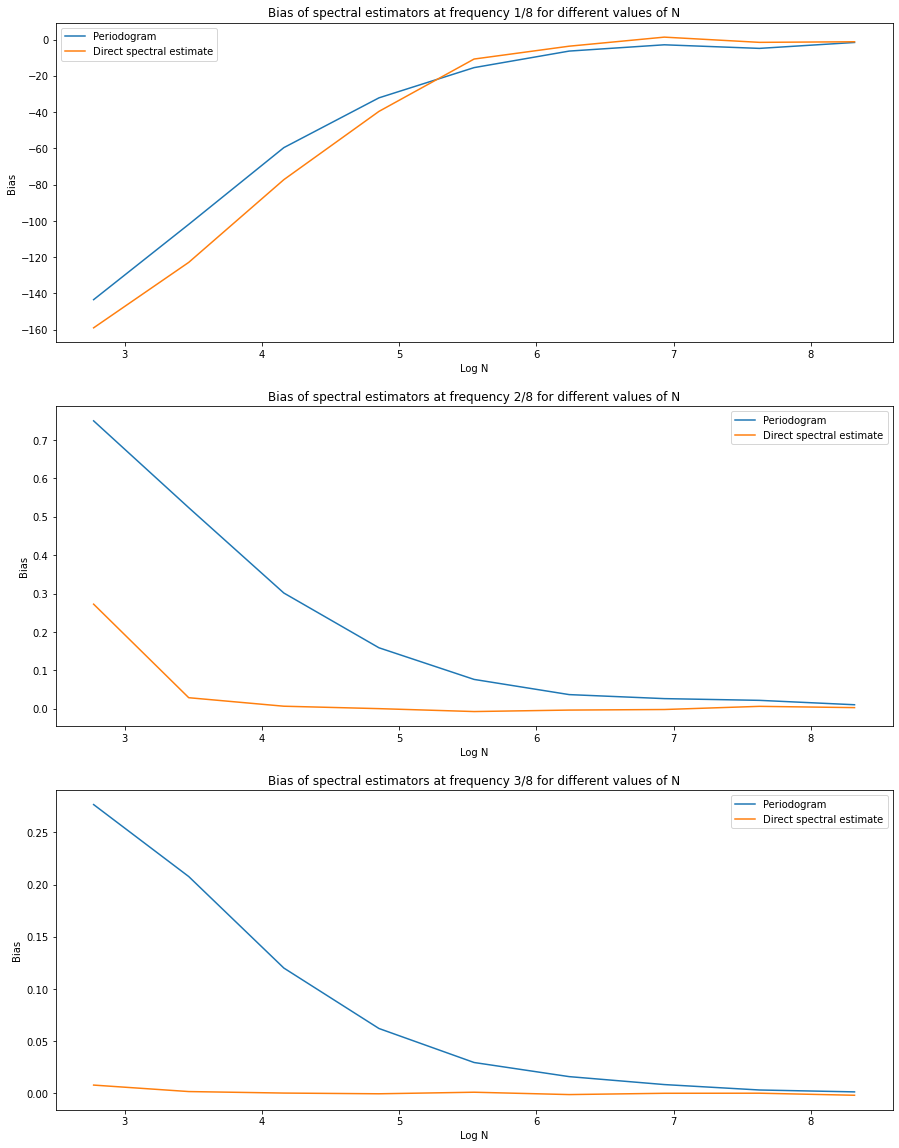
\includegraphics[width=0.9\columnwidth]{plot2b.png}
    \caption{Plot of biases for question 2(b)}
    \label{plot2b}
\end{figure}

\begin{figure}
    \centering
    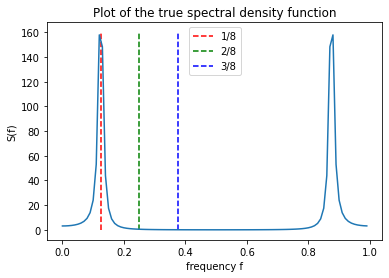
\includegraphics{plot2c.png}
    \caption{Plot of the true spectral density for question 2(c)}
    \label{plot2c}
\end{figure}

\begin{lstlisting}
def question2c():
    """
    Code for question 2c
    """
    #Compute true spectral density
    phis = np.array([0.95*2**0.5, -0.95**2])
    f_l = [i/100 for i in range(100)]
    S = S_AR(f_l, phis, 1)
    #plots
    plt.plot(f_l,S)
    plt.vlines(1/8, 0, 160, color = 'r', linestyles = 'dashed', label = '1/8' )
    plt.vlines(2/8, 0, 160, color = 'g', linestyles = 'dashed', label = '2/8' )
    plt.vlines(3/8, 0, 160, color = 'b', linestyles = 'dashed', label = '3/8' )
    plt.legend()
    plt.xlabel('frequency f')
    plt.ylabel('S(f)')
    plt.title('Plot of the true spectral density function')
    plt.show()
    return None
\end{lstlisting}
\clearpage


\section*{Question 3}
\subsection*{(a)}

Figure \ref{plot3a} shows the plots of the periodogram and the direct spectral estimate using the Hanning taper of my time series. The code is the same as \texttt{periodogram} and \texttt{direct} from question 2(a), but with an added \texttt{fftshift} to get the spectral density estimate on frequencies $[-1/2, 1/2]$.

\begin{figure}[h!]
    \centering
    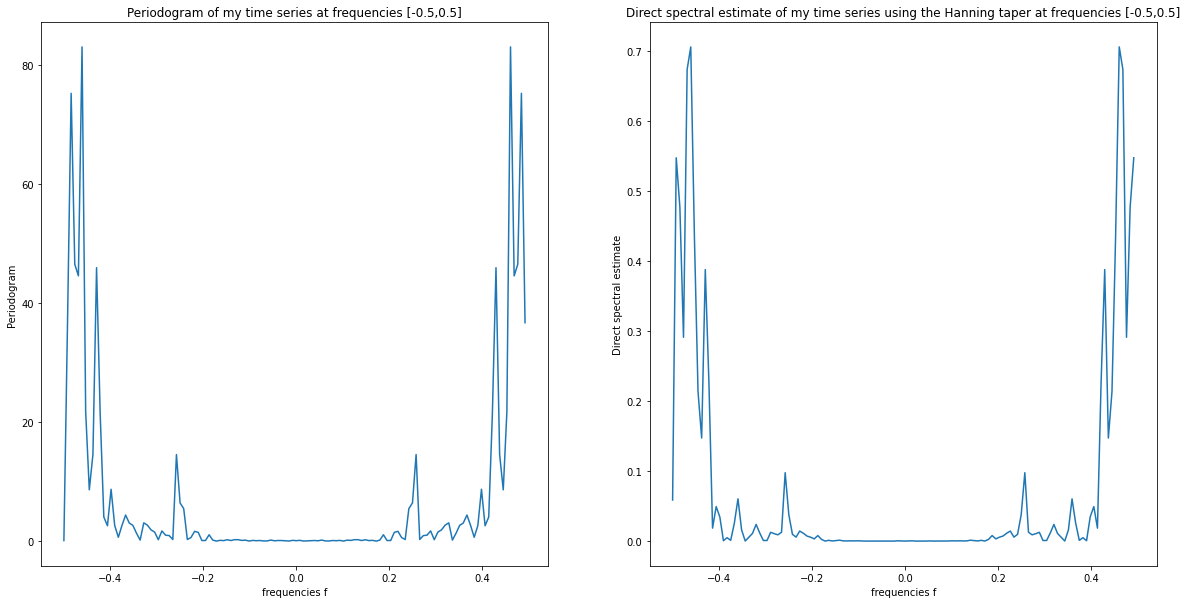
\includegraphics[width=\columnwidth]{plot3a.png}
    \caption{Plots of spectral density estimates for question 3(a)}
    \label{plot3a}
\end{figure}

\begin{lstlisting}
def question3a(X):
    """
    Code for question 3a 
    INPUT:
        X: my time series
    """
    N = len(X)
    #compute periodogram with fftshift
    S_p = (1/N)*np.abs(fftshift(fft(X)))**2
    
    #Compute tapered direct spectral estimate with fftshift
    t = np.array(range(1,N+1))
    h = 0.5*(8/(3*(N+1)))**0.5 * (1-np.cos(2*np.pi*t/(N+1)))
    
    S_d = (1/N)*np.abs(fftshift(fft(np.multiply(h,X))))**2
    
    
    #Plots
    f = [i/128 for i in range(-64,64)]
    plt.figure(figsize = (20,10))
    plt.subplot(121)
    plt.plot(f, S_p)
    plt.xlabel('frequencies f')
    plt.ylabel('Periodogram')
    plt.title('Periodogram of my time series at frequencies [-0.5,0.5]')
    
    plt.subplot(122)
    plt.plot(f, S_d)
    plt.xlabel('frequencies f')
    plt.ylabel('Direct spectral estimate')
    plt.title('Direct spectral estimate of my time series using the Hanning taper'
              +' at frequencies [-0.5,0.5]')
    plt.show() 
    return None       
\end{lstlisting}
\subsection*{(b)}

The following is my code for fitting a AR(p) model using the Yule-Walker, Least Squares and approximate maximum likelihood methods, from formulas in lecture notes.

For the Least Squares fitting, we assume w.l.o.g that $F^TF$ is invertible. 

\begin{lstlisting}
def yule_walker(X,p):
    """
    INPUT:
        X: time series of length 128
        p: order of AR(p) process that we want to fit to X
    OUTPUT:
        phi_hat = (big gamma)^-1 * small gamma, yule-walker estimator of AR(p)
        parameters phis
        sigma2_hat:  yule-walker estimator of variance of white noise process
    """
    s_hat = acvs_hat(X, list(range(0,p+1))) #estimate autocovariance sequence
    gamma = s_hat[1:] #define small gamma = [shat_1, ..., shat_p]
    #define big gamma, which is a symmetric Toeplitz matrix
    Gamma = toeplitz(s_hat[:-1], s_hat[:-1]) 
    #compute phi_hat and sigma2_hat
    phi_hat = np.linalg.inv(Gamma).dot(gamma)
    sigma2_hat = s_hat[0] - np.dot(phi_hat,s_hat[1:])
    
    return phi_hat, sigma2_hat

def least_squares(X,p):
    """
    INPUT:
        X: time series of length 128
        p: order of AR(p) process that we want to fit to X
    OUTPUT:
        phis_hat = (F.T F)^-1 F.T X, least squares estimator of AR(p) parameters phis
        sigma2_hat:  lest squares estimator of variance of white noise process
    """
    N = len(X)
    #initialise matrix F
    F = np.zeros((N-p,p))
    for i in range(p):
        # Loop to define each column of F
        F[:,i] = X[(p-i-1):(N-1-i)]
    #Compute phi_hat
    phi_hat = np.linalg.inv(F.T.dot(F)).dot(F.T).dot(X[p:])
    #Compute sigma2_hat
    sigma2_hat = (1/(N-2*p))*(X[p:]-F.dot(phi_hat)).T.dot(X[p:]-F.dot(phi_hat))
    
    return phi_hat, sigma2_hat

def approx_mle(X,p):
    """
    INPUT:
        X: time series of length 128
        p: order of AR(p) process that we want to fit to X
    OUTPUT:
        phis_hat: least squares estimator of AR(p) parameters phis (which is 
        equal to Approximate MLE)
        sigma2_hat:  approximate maximum likelihood estimator of sigma2, which
        is the lest squares estimator of sigma2 *(N-2p)/(N-p)
    """
    N = len(X)
    #Get least squares estimators of phi and sigma2
    phi_hat, sigma2_hat = least_squares(X, p)
    #Transform least squares estimator of sigma2 into approximate MLE
    sigma2_hat = sigma2_hat *(N-2*p)/(N-p)
    
    return phi_hat, sigma2_hat
\end{lstlisting}

\subsection*{(c)}

The AIC for each fitting method and process order is summarised in the table below. \\

\begin{tabular}{lrrr}
\toprule
{} &  Yule-Walker &  Least Squares &  Approximate MLE \\
\midrule
p = 1  &    83.457568 &      79.308525 &        78.296662 \\
p = 2  &    67.210892 &      62.744916 &        60.696873 \\
p = 3  &    42.897565 &      35.014882 &        31.905417 \\
p = 4  &    10.712505 &     -22.692807 &       -26.889905 \\
p = 5  &    11.667585 &     -23.526619 &       -28.838585 \\
p = 6  &    12.558746 &     -19.564828 &       -26.019978 \\
p = 7  &    13.945686 &     -16.908833 &       -24.536622 \\
p = 8  &    15.673155 &     -13.065779 &       -21.896866 \\
p = 9  &    16.615987 &     -11.939696 &       -22.006017 \\
p = 10 &    18.121540 &     -11.858851 &       -23.193686 \\
p = 11 &    19.796076 &      -7.995110 &       -20.633170 \\
p = 12 &    21.759412 &      -7.187960 &       -21.165469 \\
p = 13 &    22.142904 &      -5.101213 &       -20.456005 \\
p = 14 &    23.842761 &      -3.255814 &       -20.027431 \\
p = 15 &    25.429476 &       0.521702 &       -17.708102 \\
p = 16 &    26.306425 &       2.717655 &       -17.013632 \\
p = 17 &    26.731132 &       3.343002 &       -17.935132 \\
p = 18 &    28.727868 &       5.515377 &       -17.357172 \\
p = 19 &    30.279313 &       8.161516 &       -16.355375 \\
p = 20 &    31.917098 &      12.468884 &       -13.744801 \\
\bottomrule
\end{tabular} \\

\begin{lstlisting}
def question3c(X):
    """
    Code for question 3c
    INPUT:
        X: my time series
    OUTPUT:
        data_AIC: dataframe of AIC scores for each method and process order
    """
    #Initialise matrix of AICS
    AIC = np.zeros((20,3))
    N = len(X)
    for p in range(1,21):
        #Loop for computing AIC at each order p
        _, s_y = yule_walker(X, p)
        _, s_l = least_squares(X, p)
        _, s_m = approx_mle(X, p)
        sigma2s = np.array([s_y, s_l, s_m])
        ps = np.array([p, p, p])
        AIC[p-1,:] = 2*ps.T + N*np.log(sigma2s.T)
    
    #Summarise in a pandas DataFrame
    data_AIC = pd.DataFrame(data = AIC, 
                            index = ["p = "+ str(i) for i in range(1,21)],
                            columns = ['Yule-Walker', 
                                       'Least Squares', 'Approximate MLE'])
    
    return data_AIC
\end{lstlisting}

\subsection*{(d)}
We choose the order of model with the lowest AIC score for each fitting method.

Hence we choose $p = 4$ for the Yule-Walker model, and $p=5$ for both the Least Squares and approximate maximum likelihood models.

The corresponding parameter estimates are shown in the table below, up to 4 decimal points. \\

\begin{tabular}{lrrr}
\toprule
{} &Yule-Walker & Least Squares & Approximate MLE \\
\midrule
$\hat{\mathbf{\phi}}$    &  \parbox{3cm}{[-1.5452, -1.2955, -1.0781, -0.4841]} &  \parbox{3.75cm}{[-1.7241, -1.6180, -1.4260, -0.7367, -0.0647]} &  \parbox{3.75cm}{[-1.7241, -1.6180, -1.4260, -0.7367, -0.0647]} \\
$\hat{\sigma}^2$ &  1.0214 &  0.7696 &  0.7383 \\
\bottomrule
\end{tabular} \\

\begin{lstlisting}
def question3d(X):
    """
    Code for question 3d
    INPUT: 
        X: my time series
    OUTPUT: 
        data_params: dataframe of p+1 parameters for each method
    """
    #Compute fitted parameters for chosen p
    py, sy = yule_walker(X,4)
    pl,sl = least_squares(X, 5)
    pm,sm = approx_mle(X, 5)
    
    #Summarise parameters into a pandas DataFrame
    data_params = pd.DataFrame(data = [[ py, pl, pm],
                                       [sy, sl, sm]],
                               index = ['phi_hat', 'sigma2_hat'],
                               columns = ['Yule-Walker', 
                                       'Least Squares', 'Approximate MLE'])
    return data_params
\end{lstlisting}

\subsection*{(e)}

Figure \ref{plot3e} shows the associated spectral density function for each of the three selected models.

\begin{lstlisting}
def question 3e(X):
    """
    Code for question 3e
    INPUT:
        X: my time series
    OUTPUT: 
        py, pl, pm: phi parameters for each method
    """
    #Compute fitted parameters for chosen p
    py, sy = yule_walker(X,4)
    pl,sl = least_squares(X, 5)
    pm,sm = approx_mle(X, 5)
    
    #Compute spectral densities
    f = [i/128 for i in range(-64,65)]
    S_y = S_AR(f, py, sy)
    S_l = S_AR(f, pl, sl)
    S_m = S_AR(f, pm, sm)
    
    #plots
    fig, ax = plt.subplots(3, 1, sharex = True, sharey = True, figsize = (7,10))

    ax[0].plot(f, S_y, label = 'Yule-Walker')
    ax[0].set_title('Yule-Walker')
    ax[1].plot(f, S_l, label = 'Least Squares')
    ax[1].set_title('Least Squares')
    ax[2].plot(f, S_m, label = 'Approximate MLE')
    ax[2].set_title('Approximate MLE')
    fig.suptitle('Associated spectral density functions for each model',
                 size = 16)
    fig.text(0.5, 0.04, 'Frequencies f', va='center', ha='center')
    fig.text(0.04, 0.5, 'Spectral density', va='center', ha='center', 
             rotation='vertical')
    plt.show()
    
    return py, pl, pm
\end{lstlisting}

\begin{figure}[h!]
    \centering
    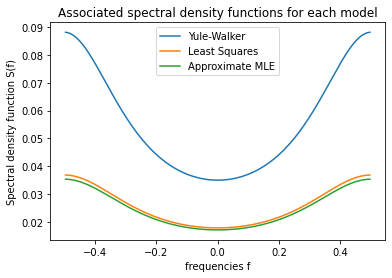
\includegraphics[width = 0.6\columnwidth]{plot_3e.png}
    \caption{Plot of spectral densities for question 3(e)}
    \label{plot3e}
\end{figure}

\clearpage
\section*{Question 4}

The table below comapres the actual values $X_119,...,  X_128$ to the forecast values, using the model parameters obtained from YW, LS and ML in question 3. I used the formula
\begin{align*}
    X_t(l) = \phi_{1,p}X_t + .. \phi_{p,p}X_{t-p+1}
\end{align*}
from lecture notes to calculate each AR(p) forecast. \\

\begin{tabular}{lrrrr}
\toprule
{} &  Actual values &  Yule-Walker &  Least Squares &   Approximate ML \\
\midrule
t = 110 & -3.73160 & -3.731600 & -3.731600 & -3.731600 \\
t = 111 &  2.14740 &  2.147400 &  2.147400 &  2.147400 \\
t = 112 & -1.69030 & -1.690300 & -1.690300 & -1.690300 \\
t = 113 &  2.23870 &  2.238700 &  2.238700 &  2.238700 \\
t = 114 & -2.21710 & -2.217100 & -2.217100 & -2.217100 \\
t = 115 &  1.72930 &  1.729300 &  1.729300 &  1.729300 \\
t = 116 & -1.18780 & -1.187800 & -1.187800 & -1.187800 \\
t = 117 &  0.26944 &  0.269440 &  0.269440 &  0.269440 \\
t = 118 &  1.76370 &  1.763700 &  1.763700 &  1.763700 \\
t = 119 & -3.49900 & -2.630999 & -2.913407 & -2.913407 \\
t = 120 &  3.66870 &  2.065189 &  2.548070 &  2.548070 \\
t = 121 & -4.21590 & -1.814666 & -2.315649 & -2.315649 \\
t = 122 &  4.40100 &  2.111316 &  2.707106 &  2.707106 \\
t = 123 & -3.80270 & -1.864365 & -2.521683 & -2.521683 \\
t = 124 &  2.50420 &  1.102283 &  1.580764 &  1.580764 \\
t = 125 &  0.36910 & -0.685727 & -0.964388 & -0.964388 \\
t = 126 & -2.37090 &  0.619468 &  0.856305 &  0.856305 \\
t = 127 &  2.95990 & -0.354670 & -0.487489 & -0.487489 \\
t = 128 & -3.26850 & -0.048823 & -0.171230 & -0.171230 \\
\bottomrule
\end{tabular} \\

Figure \ref{plot4} shows the plot of the forecast values against the true values for time points 110 to 128. Because the Least Squares and approximate ML methods give the same estimates of $\phi_{i,p}$, the forecast values are the same so the plots overlap.

\begin{figure}
    \centering
    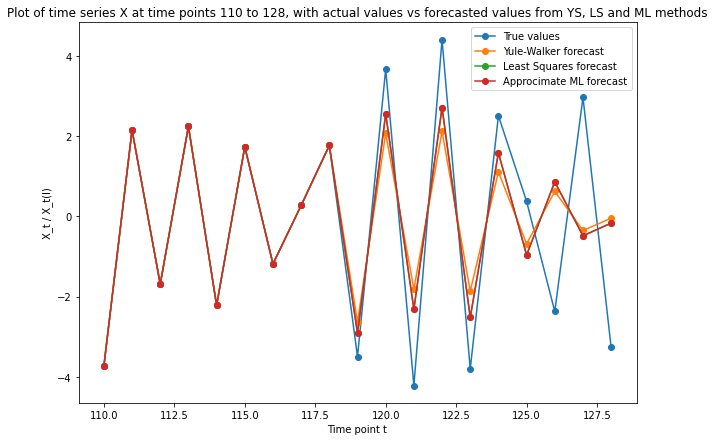
\includegraphics[width = 0.9\columnwidth]{plot4.png}
    \caption{Plot of forecast values for question 4}
    \label{plot4}
\end{figure}

\begin{lstlisting}
def question4(X):
    """
    Code for question 4
    INPUT:
        X: my time series
    OUTPUT:
        data_f: dataframe of actual and forecast values at time points 110 to 128
    """
    #Get fitted parameters
    py, pl, pm = question3e(X)
    
    #Create matrix to contain actual and forecast values
    X_f = np.zeros((128,4))
    X_f[:,0] = X
    X_f[:118,1] = X[:118]
    X_f[:118,2] = X[:118]
    X_f[:118,3] = X[:118]
    for i in range(9):
        #Loop to calculate forecast values for each method
        X_f[118 + i,1] = py[0]*X_f[118 + i-1,1] +py[1]*X_f[118 + i-2,1] \
            + py[2]*X_f[118 + i-3,1]+ py[3]*X_f[118 + i-4,1]
            
        X_f[118 + i,2] = pl[0]*X_f[118 + i-1,2] +pl[1]*X_f[118 + i-2,2] \
            + pl[2]*X_f[118 + i-3,2]+ pl[3]*X_f[118 + i-4,2] \
                + pl[4]*X_f[118 + i-5,2]
            
        X_f[118 + i,3] = pm[0]*X_f[118 + i-1,3] +pm[1]*X_f[118 + i-2,3] \
            + pm[2]*X_f[118 + i-3,3]+ pm[3]*X_f[118 + i-4,3] \
                + pm[4]*X_f[118 + i-5,3]
                
    #take values only from time point 110
    X_f = X_f[109:,:]
    
    #Plots
    t = [i for i in range(110, 129)]
    plt.figure(figsize = (10,7))
    plt.plot(t, X_f[:,0], label = 'True values', marker = 'o')
    plt.plot(t, X_f[:,1], label = 'Yule-Walker forecast', marker = 'o')
    plt.plot(t, X_f[:,2], label = 'Least Squares forecast', marker = 'o')
    plt.plot(t, X_f[:,3], label = 'Approcimate ML forecast', marker = 'o')
    plt.legend()
    plt.title('Plot of time series X at time points 110 to 128, with actual '+
              'values vs forecasted values from YS, LS and ML methods')
    plt.xlabel('Time point t')
    plt.ylabel('X_t / X_t(l)')
    plt.show()
    
    #summarise forecast and actual values into pandas Data Frame
    data_f = pd.DataFrame(X_f, index = ['t = '+str(i) for i in range(110,129)],
                          columns = ['Actual values', 'Yule-Walker', 
                                     'Least Squares', ' Approximate ML'])
    return data_f
\end{lstlisting}
\end{document}
